\documentclass[11pt, pdftex, final]{styles/change}

%%%%%%%%%%%%%%%%%%%%%%%%%%%%%%%%%%%%%%%%%%%%%%%%%%%%%%%%%%%%%%%%%%%%%%
%                 Includes
%%%%%%%%%%%%%%%%%%%%%%%%%%%%%%%%%%%%%%%%%%%%%%%%%%%%%%%%%%%%%%%%%%%%%%
\usepackage[utf8x]{inputenc}
\usepackage[pdftex]{graphicx}
\usepackage[pdftex,usenames,dvipsnames]{color}
\usepackage{epstopdf}
\usepackage{dirtree}
\usepackage{listings}
\usepackage{xcolor}


% \usepackage[pdftex,
%            pdfpagelabels,
%            plainpages=false,
%            hypertexnames=false,
%            pdffitwindow=true,      % page fit to window when opened
%            colorlinks=true,
%            linkcolor=blue,
%            urlcolor=blue,
%            pdfauthor={CHANGE consortium},
%            pdftitle={CHANGE consortium Deliverable},
%            pdfproducer={Latex with hyperref},
%            pdfcreator={pdflatex}
%           ]{hyperref}

\usepackage[colorlinks]{hyperref}
\usepackage{xspace}
%\usepackeage{}

%\usepackage{draftcopy}
\usepackage{epsfig}
\usepackage{algorithmic}
\usepackage[ruled,linesnumbered]{algorithm2e}
 
\usepackage[subfigure, titles] {tocloft}
\usepackage{subfigure}
\usepackage{stdclsdv}
\usepackage{fancyhdr, lastpage}
\usepackage{supertabular}
\usepackage{hhline}
\usepackage{multirow}
\usepackage{amsmath, amssymb, amsbsy, amsthm}
\usepackage{bm}
\usepackage{calc}

\usepackage[nonumberlist,acronym,toc,style=altlist,]{glossaries}
%% use for a symbols table 
\newglossary[slg]{symbols}{sym}{sbl}{List of Symbols}
\makeglossary


% % mahmed only use in draft mode 
% %\usepackage[verbose]{geometry}


%%%%%%%%%%%%%%%%%%%%%%%%%%%%%%%%%%%%%%%%%%%%%%%%%%%%%%%%%%%%%%%%%%%%%%%
% Replace the standard Computer Modern Typewriter font LaTeX uses for %
% monospace text with the PostScript font Adobe Courier.              %
%%%%%%%%%%%%%%%%%%%%%%%%%%%%%%%%%%%%%%%%%%%%%%%%%%%%%%%%%%%%%%%%%%%%%%%
\usepackage{courier}

%%%%%%%%%%%%%%%%%%%%%%%%%%%%%%%%%%%%%%%%%%%%%%%%%%%%%%%%%%%%%%%%%%%%%
% Allow relative font size specifications (e.g. \smaller, \larger). %
%%%%%%%%%%%%%%%%%%%%%%%%%%%%%%%%%%%%%%%%%%%%%%%%%%%%%%%%%%%%%%%%%%%%%
\usepackage{relsize, setspace}
\usepackage{marginnote}




%%%%%%%%%%%%%%%%%%%%%%%%%%%%%%%%%%%%%%%%%%%%%%%%%%%%%%%%%%%%%%%%%%%
% Control the fonts and formatting used in the table of contents. %
% and  Use Helvetica-Narrow Bold for Chapter entries              %
%%%%%%%%%%%%%%%%%%%%%%%%%%%%%%%%%%%%%%%%%%%%%%%%%%%%%%%%%%%%%%%%%%%
\usepackage[titles]{tocloft}
\renewcommand{\cftchapfont}{%
  \fontsize{11}{13}\usefont{OT1}{phv}{bc}{n}\selectfont }

%%%%%%%%%%%%%%%%%%%%%%%%%%%%%%%%%%%%%%%%%%%%%%%%%%%%%%%%%%%%%%%%%%%%%%%%
% Cleveref - used to replace \ref and \autoref                         %
% http://www.ctan.org/tex-archive/help/Catalogue/entries/cleveref.html %
% mahmed: Load this last                                               %
%%%%%%%%%%%%%%%%%%%%%%%%%%%%%%%%%%%%%%%%%%%%%%%%%%%%%%%%%%%%%%%%%%%%%%%%
% \usepackage{cleveref}



%%%%%%%%%%%%%%%%%%%%%%%%%%%%%%%%%%%%%%%%%%%%%%%%%%%%%%%%%%%%%%%%%%%%%%%%
%                 Input the latex macros%
%%%%%%%%%%%%%%%%%%%%%%%%%%%%%%%%%%%%%%%%%%%%%%%%%%%%%%%%%%%%%%%%%%%%%%%%

\def\consortiumName {Universitatea POLITEHNICA din București \\
și \\
ORANGE România S.A.}
\def\consortiumNameChange {}
\def\change {\consortiumNameChange\ }
\def\consortiumICT {Contract nr.23\/2017}

\def\consortiumLogoLarge{
\includegraphics[width=2.25cm]{figures/upb-logo.png}
  
\includegraphics[width=2.25cm]{figures/orange-logo.png}}
\def\consortiumLogoSmall{
\includegraphics[width=1.25cm]{figures/upb-logo.png}

\includegraphics[width=1.25cm]{figures/orange-logo.png}}
\def\fp7LogoLarge{}
%
\includegraphics[width=2.5cm]{styles/images/fp7-logo-large}}

\def\documentNumbering {Page \thepage\ of (\pageref{LastPage})}
\def\documentCopyright {\copyright\ \consortiumName\ \the\year\ }


\docConfidential{
%%   \noindent\textbf{Disclaimer}\\
%%   This document contains material, which is
%%   copyright of certain CHANGE consortium parties and may not be reproduced or
%%   copied without permission. The information contained in this document is the
%%   proprietary confidential information of certain CHANGE consortium parties and
%%   may not be disclosed except in accordance with the consortium agreement.  \\ 
%%   The commercial use of any information in this document may require a license
%%   from the proprietor of that information. \\ 
%%   Neither the CHANGE consortium as a whole, nor a certain party of the CHANGE
%%   consortium warrant that the information contained in this document is capable
%%   of use, or that use of the information is free from risk, and accept no
%%   liability for loss or damage suffered by any person using the information.
%%   This document does not represent the opinion of the European Community, and the
%%   European Community is not responsible for any use that might be made of its
%%   content. 
}

\docPublic{
%%   \noindent\textbf{Disclaimer}\\
%%   This document contains material, which is the copyright of certain CHANGE
%%   consortium parties, and may not be reproduced or copied without permission. All
%%   CHANGE consortium parties have agreed to the full publication of this
%%   document. The commercial use of any information contained in this document may
%%   require a license from the proprietor of that information.\\
%%   Neither the CHANGE consortium as a whole, nor a certain party of the CHANGE
%%   consortium warrant that the information contained in this document is capable
%%   of use, or that use of the information is free from risk, and accept no
%%   liability
%%   for loss or damage suffered by any person using this information.\\
%%   This document does not represent the opinion of the European Community, and the
%%   European Community is not responsible for any use that might be made of its
%%   content.  
}

\def\documentImpressum{
%%   \begin{tabular} {p{4.25cm}p{11.0cm}}
%%     \multicolumn{2}{l}{\textbf{Impressum}} \\ 
%%     Full project title        & CHANGE: Enabling Innovation in the Internet 
%%                              Architecture through Flexible Flow-Processing 
%%                              Extensions \\ 
%%     Title of the workpackage  & Dx.y  document title \\
%%     Editor                    & Name, company \\
%%     Project Co-ordinator      & Adam Kapovits, Eurescom\\
%%     Technical Manager         & Felipe Huici, NEC\\
%%     \textbf{Copyright notice} & \copyright\ \the\year\ Participants in project \consortiumName\ \\
%%   \end{tabular}    
}


% \fancypagestyle{plain}{%
% \fancyhf{} % clear all header and footer fields
% \fancyfoot[C]{\bfseries \thepage} % except the center
% \renewcommand{\headrulewidth}{0pt}
% \renewcommand{\footrulewidth}{0pt}}

\fancypagestyle{changeFrontPage}{%
\fancyhf{} % clear all header and footer fields
\lhead{\consortiumLogoLarge}
\rhead{\fp7LogoLarge}
\lfoot{\footnotesize{\documentCopyright\ } }
\rfoot{\footnotesize{\documentNumbering\ }} %
\renewcommand{\headrulewidth}{0.4pt}
\renewcommand{\footrulewidth}{0.4pt}}


%% header and footer                                   %
\pagestyle{fancy}                                      %
\fancyhead{} % clear all header fields                 %
\fancyhead[RE,LO]{\consortiumLogoSmall}                %
\fancyhead[RO,LE]{\documentTitle}                      %
\fancyfoot{} % clear all footer fields                 %
\fancyfoot[RO,LE]{\footnotesize{\documentNumbering\ }} %
\fancyfoot[RE,LO]{\footnotesize{\documentCopyright\ }} %
\renewcommand{\headrulewidth}{0.4pt}                   %
\renewcommand{\footrulewidth}{0.4pt}                   %






%%%%%%%%%%%%%%%%%%%%%%%%%%%%%%%%%%%%%%%%%%%%%%%%%%%%%%%%%%%%%%%%%%%%%%
%%% changeGlobalDefs.tex ends here

%%% Local Variables: 
%%% mode: latex
%%% TeX-master: t
%%% End: 

%% %%%%%%%%%%%%%%%%%%%%%%%%%%%%%%%%%%%%%%%%%%%%
% Lower-case Roman syle enumeration count  %
%%%%%%%%%%%%%%%%%%%%%%%%%%%%%%%%%%%%%%%%%%%%
\renewcommand{\labelenumi}{(\roman{enumi})}
\renewcommand{\labelenumii}{(\roman{enumi}.\alph{enumii})}
\renewcommand{\labelenumii}{(\alph{enumii})}

%%%%%%%%%%%
% Colours %
%%%%%%%%%%%
\definecolor{Brown}{cmyk}{0,0.81,1,0.60}
\definecolor{OliveGreen}{cmyk}{0.64,0,0.95,0.40}
\definecolor{CadetBlue}{cmyk}{0.62,0.57,0.23,0}
\definecolor{Grey}{cmyk}{0,0,0,0.10}
\definecolor{Light}{gray}{.80}

%%%%%%%%%%%
% More standardised \ref definitions 
%%%%%%%%%%%
%%
\crefname{algorithm}{algorithm}{algorithms}
\Crefname{algorithm}{Algorithm}{Algorithms}

%\crefname{algocf}{alg.}{algs.}
%\Crefname{algocf}{Algorithm}{Algorithms}

\crefformat{algorithm}{Alg.~(#2#1#3)}
\Crefformat{algorithm}{Algorithm~(#2#1#3)}

\crefmultiformat{algorithm}{Algs.~(#2#1#3)}%
  { and~(#2#1#3)}{, (#2#1#3)}{ and~(#2#1#3)}
\Crefmultiformat{algorithm}{Algorithms~(#2#1#3)}%
  { and~(#2#1#3)}{, (#2#1#3)}{ and~(#2#1#3)}

%%
\crefformat{equation}{Eq.~(#2#1#3)}
\Crefformat{equation}{Equation~(#2#1#3)}

\crefmultiformat{equation}{Eqs.~(#2#1#3)}%
  { and~(#2#1#3)}{, (#2#1#3)}{ and~(#2#1#3)}
\Crefmultiformat{equation}{Equations~(#2#1#3)}%
  { and~(#2#1#3)}{, (#2#1#3)}{ and~(#2#1#3)}

%%
\crefformat{figure}{Fig.~(#2#1#3)}
\Crefformat{figure}{Figure~(#2#1#3)}

\crefmultiformat{figure}{Figs.~(#2#1#3)}%
  { and~(#2#1#3)}{, (#2#1#3)}{ and~(#2#1#3)}
\Crefmultiformat{figure}{Figures~(#2#1#3)}%
  { and~(#2#1#3)}{, (#2#1#3)}{ and~(#2#1#3)}



%%%%%%%%%%%%%
% Theorems  %
%%%%%%%%%%%%%
\newtheorem{theorem}{Theorem} [chapter]
\newtheorem{lemma}{Lemma} [chapter]
\newtheorem{proposition}{Proposition} [chapter]
\newtheorem{conjecture}{Conjecture} [chapter]
\newtheorem{example}{Example}
\newtheorem{definition}{\textit{Definition}:}[chapter]
\newtheorem{corollary}{Corollary} [chapter]

\theoremstyle{remark}
\newtheorem*{remrk}{Remark}

\newcommand{\fig}[1]{Fig.~\autoref{#1}}



%% For background
\newcommand{\argmax}{\operatorname{argmax}}
\newcommand{\dataRate}{r}
\newcommand{\dataRateVec}{\vec{\dataRate}}
\newcommand{\lagrangeMultiplier}{q}
%\newcommand{\lagrangeMultiplierVec}{\stackrel{\rightarrow}{\lagrangeMultiplier}}
\newcommand{\lagrangeMultiplierVec}{\vec{\lagrangeMultiplier}}
\newcommand{\powerVec}{\vec{\power}}
\newcommand{\feasiblePowerAssignment}{\Pi}
\newcommand{\dataRateRegion}{{\cal {R}}}
\newcommand{\convHull}[1]{\operatorname{Co}(#1)}
\newcommand{\userRate}{x}
\newcommand{\userRateVector}{\vec{\userRate}}
\newcommand{\capacityRegion}{\Lambda}
\newcommand{\queue}{q}
\newcommand{\queueVector}{\vec{\queue}}


%%%%%%%%%%%%%%%%%%%%%%%%%%%%%%%%%%%%%%%%%%%%%%%%%%%%%%%%%%%%%%%%%%%%%%
%%% macros.tex ends here


%%%%%%%%%%%%%%%%%%%%%%%%%%%%%%%%%%%%%%%%%%%%%%%%%%%%%%%%%%%%%%%%%%%%%%
%% THE GLOSSARY
%%%%%%%%%%%%%%%%%%%%%%%%%%%%%%%%%%%%%%%%%%%%%%%%%%%%%%%%%%%%%%%%%%%%%%

% The following definitions will go in the main glossary
\newglossaryentry{culdesac}{
  name=cul-de-sac,
  description={passage or street closed at one end},
  plural=culs-de-sac
}

\newglossaryentry{elite}{
  name={\'e}lite,
  description={select group or class},
  sort=elite
}

\newglossaryentry{elitism}{
  name={\'e}litism,
  description={advocacy of dominance by an \gls{elite} },
  sort=elitism
}

\newglossaryentry{attache}{
  name=attach\'e,
  description={person with special diplomatic responsibilities}
}

% The following definitions will go in the list of acronyms
\newacronym{led}{LED}{
  light-emitting diode
}

\newacronym{eeprom}{EEPROM}{
  electrically erasable programmable
  read-only memory
}


%%%%%%%%%%%%%%%%%%%%%%%%%%%%%%%%%%%%%%%%%%%%%%%%%%%%%%%%%%%%%%
% % The following definitions will go in the list of symbols %
% \newglossaryentry{ohm}{                                    %
%   type=symbols,name=ohm,                                   %
%   symbol={\ensuremath{\Omega}},                            %
%   description=unit of electrical resistance                %
% }                                                          %
%                                                            %
% \newglossaryentry{angstrom} {                              %
%   type=symbols,name={\aa}ngstr\"om,                        %
%   symbol={\AA},sort=angstrom,                              %
%   description={non-SI unit of length}                      %
% }                                                          %
%%%%%%%%%%%%%%%%%%%%%%%%%%%%%%%%%%%%%%%%%%%%%%%%%%%%%%%%%%%%%%



%\bigskip

%%%%%%%%%%%%%%%%%%%%%%%%%%%%%%%%%%%%%%%%%%%%%%%%%%%%%%%%%%%%%%%%%%%%%%
%%% glossary.tex ends here



%%%%%%%%%%%%%%%%%%%%%%%%%%%%%%%%%%%%%%%%%%%%%%%%%%%%%%%%%%%%%%%%%%%%%%%%
%                 Start the document
%%%%%%%%%%%%%%%%%%%%%%%%%%%%%%%%%%%%%%%%%%%%%%%%%%%%%%%%%%%%%%%%%%%%%%%%
\begin{document}

%%%%%%%%%%%%%%%%%%%%%%%%%%%%%%%%%%%%%%%%%%%%%%%%%%%%%%%%%%%%%%%%%%%%%%%%
%                 Title page
%%%%%%%%%%%%%%%%%%%%%%%%%%%%%%%%%%%%%%%%%%%%%%%%%%%%%%%%%%%%%%%%%%%%%%%%

\documentTitle{Raport Științific și Tehnic: Etapa finală/2018}
\frmwrkBlurb{Proiect Experimental Demonstrativ}

\documentDueDate{\today\ } 
\documentSubmitDate {\today\ }
\projStartDate{1 Ianuarie 2017}
\projDuration{18 luni}
\delivLeadContractor{Universitatea POLITEHNICA din București și ORANGE Romania}
\delivVersion{1, 30 Iunie 2018 }
\delivConfStatus{Public}


\title{Serviciu 4.5G bazat pe MPTCP}

   

%%%%%%%%%%%%%%%%%%%%%%%%%%%%%%%%%%%%%%%%%%%%%%%%%%%%%%%%%%%%%%%%%%%%%%
%%% frontpages.tex ends here


\makeTitlePage
%\makeAbstractPage{public}


%%%%%%%%%%%%%%%%%%%%%%%%%%%%%%%%%%%%%%%%%%%%%%%%%%%%%%%%%%%%%%%%%%%%%%%%
%                 Contents included from this file
%%%%%%%%%%%%%%%%%%%%%%%%%%%%%%%%%%%%%%%%%%%%%%%%%%%%%%%%%%%%%%%%%%%%%%%%
% Make TeX less fussy about line breaking %
\sloppy

\tableofcontents
%\listoffigures
%\listoftables

% Occasionally you may find that another package defines \cleardoublepage when it
% is not required. This may cause an unwanted blank page to appear before each
% glossary. This can be fixed by redefining \glsclearpage:
% http://theoval.cmp.uea.ac.uk/~nlct/latex/packages/glossaries/glossaries-manual.html
\renewcommand*{\glsclearpage}{\clearpage}

%%%%%%%%%%%%%%%%%%%%%%%
% print the glossary  %
%%%%%%%%%%%%%%%%%%%%%%%
%\printglossary[title= Definitions,
%               toctitle=Definitions,
%               style=list,
%               ]

%%%%%%%%%%%%%%%%%%%%%%%
% print the acronyms  %
%%%%%%%%%%%%%%%%%%%%%%%
%\printglossary[type=\acronymtype,
%               title=Acronyms,
%               toctitle=Acronyms,
%               style=list
%               ]


% %%%%%%%%%%%%%%%%%%%%%%%n
% % print the symbols  %
% %%%%%%%%%%%%%%%%%%%%%%%
% \printglossary[type=symbols,
%                title=Symbols,
%                toctitle=Symbols,
%                style=list
%                ]
 
%%%%%%%%%%%%%%%%%%%%%%%%%%%%%%%%%%%%%%%%%%%%%%%%%%%%%%%%%%%%%%%%%%%%%
%% WORK STARTS HERE ......................................
%%%%%%%%%%%%%%%%%%%%%%%%%%%%%%%%%%%%%%%%%%%%%%%%%%%%%%%%%%%%%%%%%%%%%

\chapter{Rezumatul proiectului}

Proiectul 4.5G își propune implementarea unei punți între tehnologiile
curente 4G și cele emergente 5G. Această punte se realizează la
nivelul transport (TCP) prin folosirea noului protocol de transport
MPTCP pentru a utiliza în mod transparent, cumulativ si simultan
tehnologiile de rețea existente, în principal 3G/4G și WiFi, dar
potențial și alte tehnologii de comunicatie disponibile pe mobile în
viitor.


Scopul proiectului este de a instrumenta terminale Android existente,
astfel încât upgrade-ul la MPTCP nu aduce un regres de uzabilitate sau
necesitatea recompilării aplicațiilor. Avantajele aduse sunt {\bf
  conectivitatea continuă} la schimbarea rețelei WiFi sau 4G, {\bf
  capacitatea crescută} când ambele rețele sunt prezente, și {\bf
  viteză ridicată de răspuns} pentru aplicațiile interactive.


\section{ Nivel de maturitate al tehnologiilor (Tehnology Readiness Levels)}

Proiectul a demarat la nivelul TRL2, avănd beneficii clare pentru
operatori și utilizatori finali, si o literatură de specialitate care
include experimente incipiente, implementări propuse, și unele măsurători. 

Pe parcursul proiectului, mai multe etape specifice TRL3 au fost
atinse - mai multe arhitecturi de proxy au fost evaluate analitic si
experimental, arhitectura aleasă implicând folosirea RTT (round trip
time) care afectează utilizatorii.  

Livrabilul final al proiectului este un demonstrator situat la nivelul
TRL4: un telefon instrumentat și serverul proxy asociat de plasat la
operatorul 4G au fost testate într-un mnediu controlat dar realistic
la partenerul Orange Romania. Componentele au fost validate prin teste
în rețeaua 4G și WiFi, și prototipul este valid ca funcționalitate și
performanță.

\pagebreak

\section{Imagini reprezentative}

\begin{figure}[h]
	\centering
	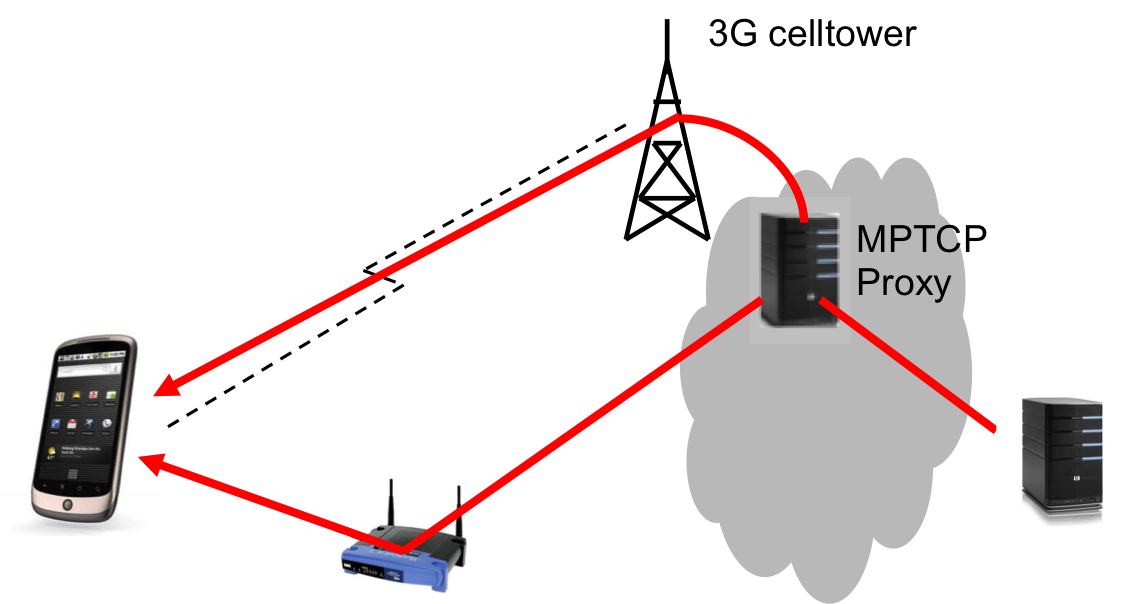
\includegraphics[scale=0.7]{figures/45g_proxy.png}
	\caption{Comunicația prin proxy}
\end{figure}


%% \begin{figure}[h]
%% 	\centering
%% 	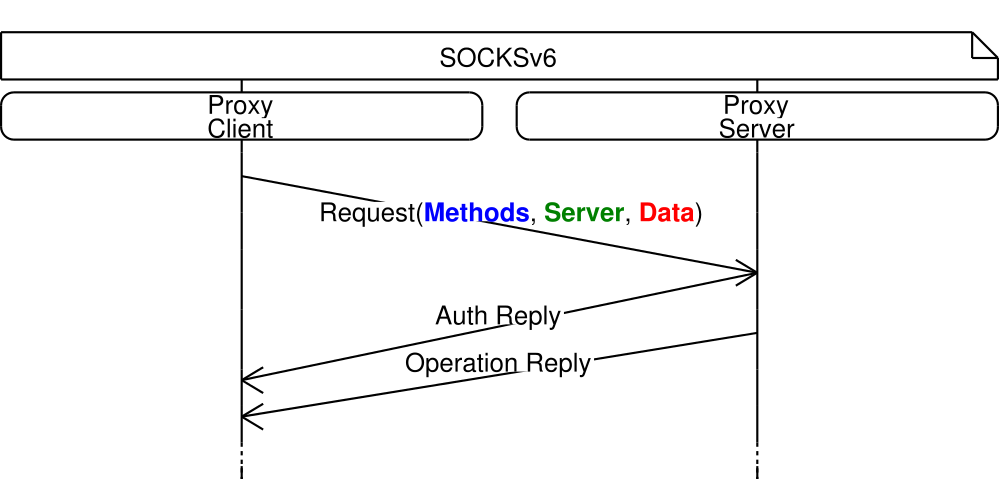
\includegraphics[scale=0.7]{figures/socks/socks6op2nd.png}
%% 	\caption{Mod de operare SOCKS 6 (conexiuni ulterioare)}
%% \end{figure}

\begin{figure}[h]
        \centering
        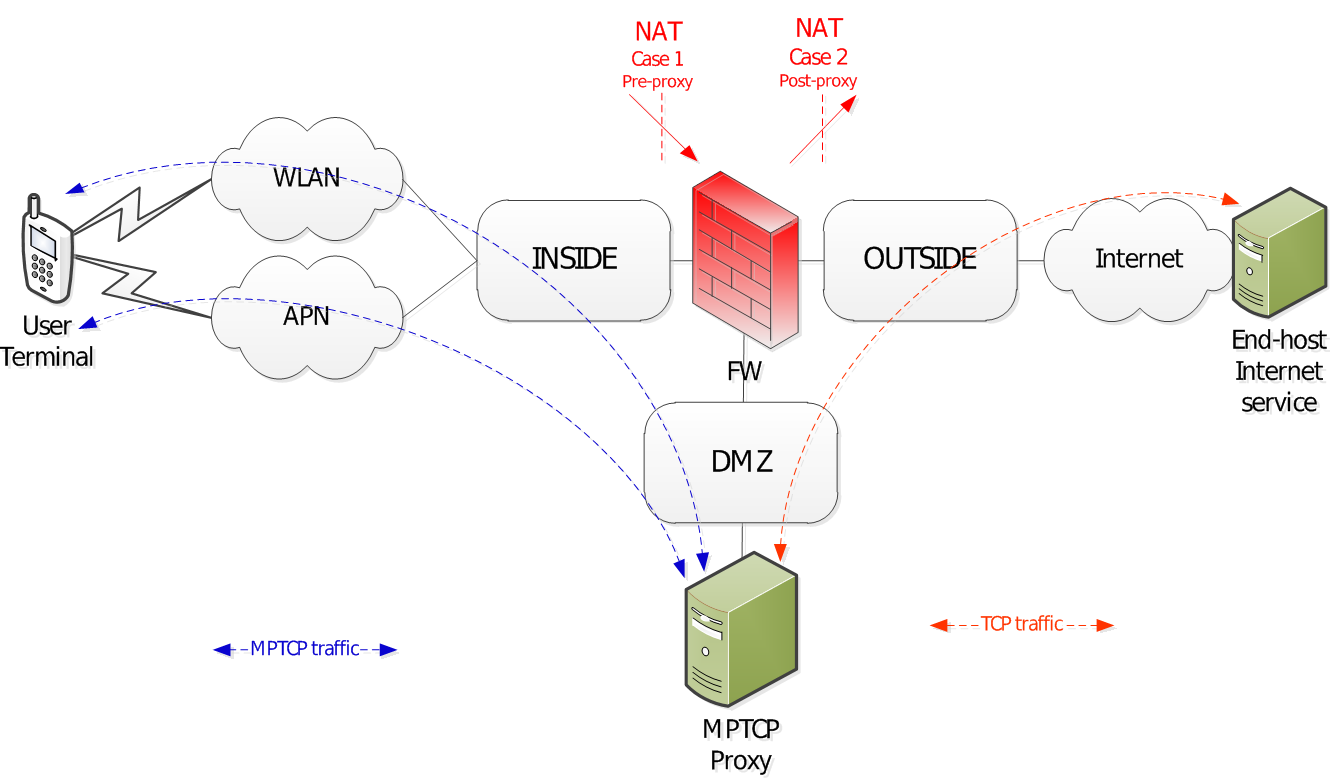
\includegraphics[scale=0.3]{figures/oro/oro_mptcp.png}
        \caption{Plasarea proxy-ului de MPTCP în rețeaua Orange Romania}
\end{figure}


 

\chapter{Obiective}
\label{sec:objectives}



\begin{itemize}
\item Implementarea modificărilor necesare pe telefoane: modificarea
kernel-ului și actualizări la Android pentru a folosi
MPTCP. Sistemul Android se bazează pe Linux, dar există suficiente
diferențe și părți specifice dispozitivului pentru a face un port
compatibil cu toate aplicațiile non-trivial.

\item Implementare și plasare proxy în rețeua Orange România
SGiLAN. Proxy-ul poate fi explicit sau transparent, fiecare soluție necesită
o implementare diferită pe telefon și la proxy.


\item Executare măsurători de performanță pentru diferite scenarii
  pentru a optimiza: conectivitatea, capacitatea, experiența cât mai
  fluidă a utilizatorului. Deoarece actualizarea MPTCP este invazivă
  pentru stiva TCP/IP, nu trebuie să existe nicio regresie a
  funcționalității sau performanțelor atunci când serviciul este
  implementat într-o rețea de testare cu o utilizatori reali.


\item Realizarea unui prototip pentru testarea la scară mai largă,
  folosind echipe de testare ale operatorului sau grupuri de
  utilizatori specializați.


\end{itemize}

\chapter{Studiu conectare MPTCP în rețeaua ORO}
\label{sec:oro_arch}

\section{Caracteristicile rețelei 3G/4G ORO}

Reţeaua ORO, prezentată în figura \ref{fig:oro_network}, oferă atât
servicii de date mobile folosind rețeaua celulară, cât şi servicii de
conectare la internet folosind reţele WiFi.  In cazul reţelei 3G/4G,
accesul se face prin echipamentele NodeB, RNC, EPG pentru sesiunile
3G, respectiv eNodeB, MME, EPG pentru sesiunile 4G, iar tot traficul
este filtrat prin echipamentele de tip Firewall, de unde se face
accesul către internet.  Orange Romania oferă si rețele Wi-Fi pentru
accesul la internet, folosindu-se de echipamente de tip Access Point,
iar traficul este agregat central in rețea in WLAN GW.  Clienții
folosesc un APN a primi acces la internet, iar clienții comerciali
folosesc APN-ul net. Pentru aceștia, opțiunile extra din protocolul
TCP precum MPTCP sunt tăiate de către Firewall-uri, așadar pentru
implementarea acestui serviciu de tip 4.5G sunt necesare configurarea
unui APN dedicat si configurarea si realizarea unei configurații
speciale in rețea pentru plasarea Proxy-ului MPTCP.

\begin{figure}[h]
	\centering
	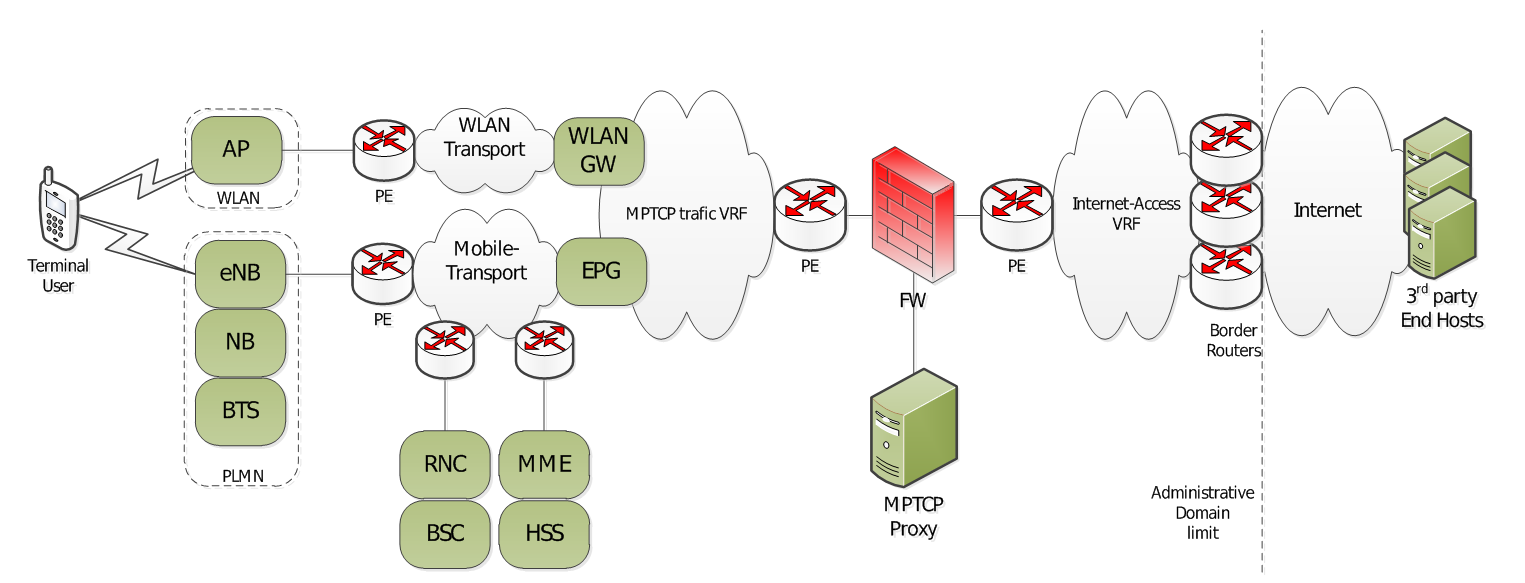
\includegraphics[scale=0.3]{figures/oro/oro_network.png}
	\caption{Structura generală a rețelei de test}
    	\label{fig:oro_network}
\end{figure}


\section{Plasarea proxy-ului MPTCP în rețeaua SGi-LAN}

\begin{figure}[h]
	\centering
	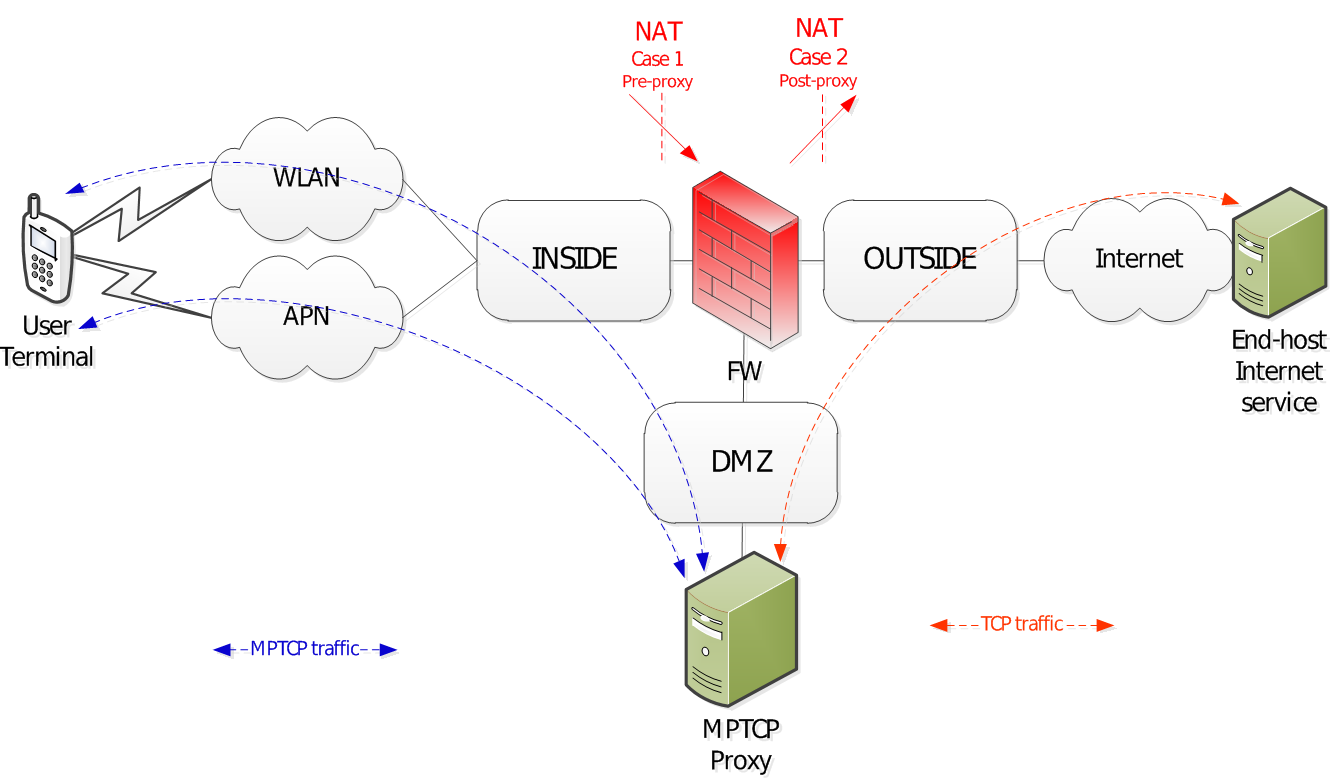
\includegraphics[scale=0.3]{figures/oro/oro_mptcp.png}
	\caption{Plasarea proxy-ului de MPTCP în spatele unui firewall cu trei zone}
    	\label{fig:oro_mptcp}
\end{figure}

Serviciul MPTCP va fi testat utilizând un APN dedicat, prin
infrastructura de date mobile și un SSID dedicat, prin intermediul
infrastructurii WLAN. Atât APN-ul, cât și SSID-ul vor folosi adresare
IP privată pentru serviciul de acces la Internet al utilizatorilor
Conectivitatea la Internet va fi asigurată folosind funcția CG-NAT44
pe un Firewall a serviciului, iar expunerea serviciilor de acces la
Internet prin intermediul unui echipament Firewall este necesară
pentru a evita intrarea pe Internet a traficului nesolicitat de la
terminalele utilizatorilor; acest trafic poate afecta autonomia
bateriilor terminalelor mobile, precum și consumul planului de date
privind abonamentele.  Se va implementa următorul design de Firewall
cu trei zone prezentat în figura \ref{fig:oro_mptcp}:
\begin{itemize}
 \item Zona FW Inside - zona APN și WLAN
 \item Zona FW DMZ -zona MPTCP Proxy
 \item Zona FW Outside- zona de internet
\end{itemize}
 
Setări pentru politica de protecție Firewall:
\begin{itemize}
 \item 	permite trafic: \\
o	Inside $\rightarrow$ DMZ\\
o	Inside  $\rightarrow$  Outside\\
o	DMZ  $\rightarrow$  Outside
\item blocarea traficului:\\
o	Outside   $\rightarrow$  Inside\\
o	Outside  $\rightarrow$  DMZ
\end{itemize}


\section{Opțiuni de instalare a funcției NAT în funcție de poziția proxy-ului de MPTCP }

Funcția de NAT va face translatarea adreselor IP private in adrese IP
publice.  Nu se va efectua traducerea adreselor pentru adresa IP de
destinație către Proxy sau Internet.  Din perspectiva dispozitivului
NAT există două opțiuni de instalare a funcției NAT:
 \\

\begin{figure}[h]
	\centering
	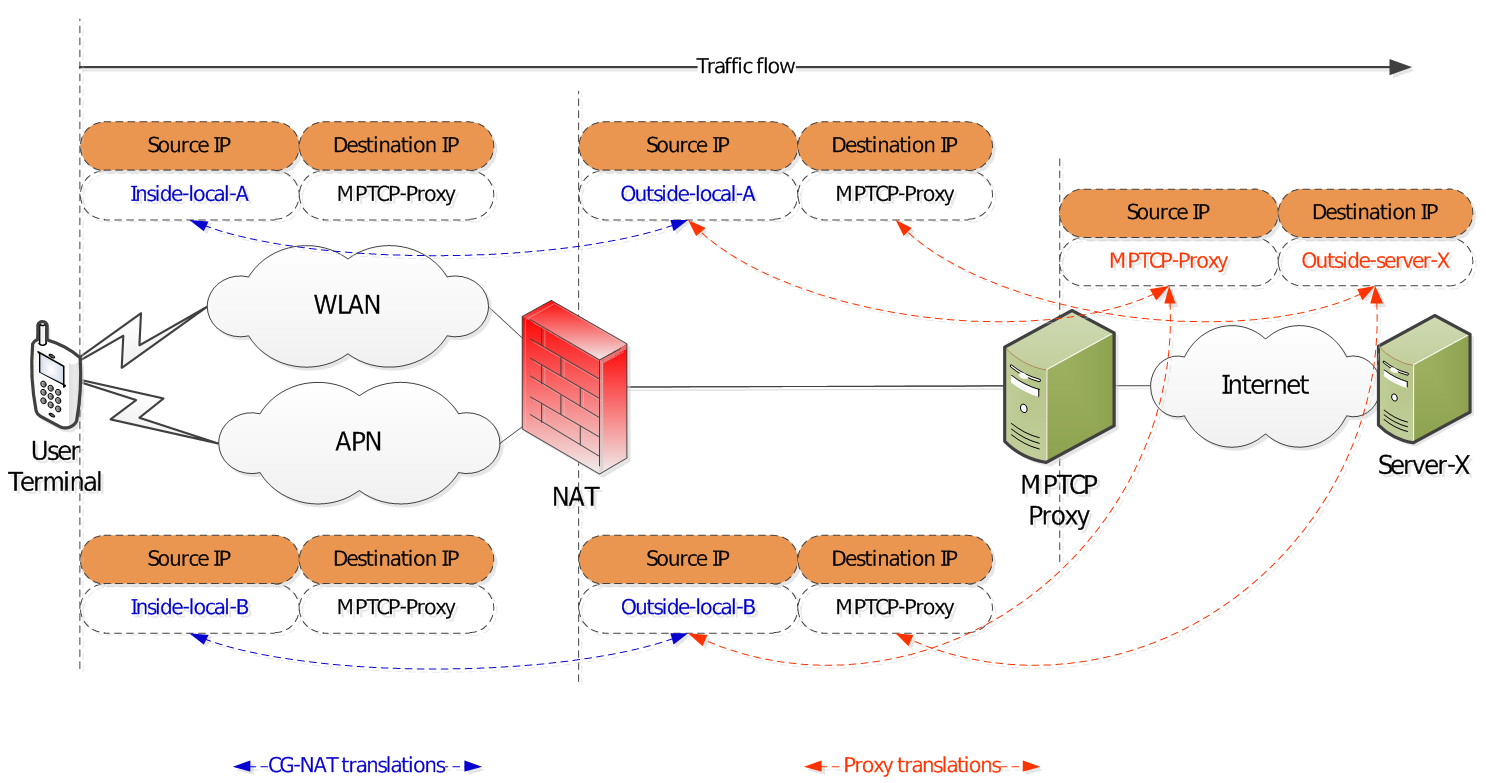
\includegraphics[scale=0.3]{figures/oro/oro_mptcp_nat.png}
	\caption{Pre-proxy NAT}
    	\label{fig:oro_mptcp_nat}
\end{figure}



{\em Cazul 1}: (figura \ref{fig:oro_mptcp_nat}) Pre-Proxy NAT – funcția NAT este plasata intre terminal si MPTCP Proxy.
\begin{itemize}
 \item	Proxy-ul trebuie să fie configurat cu o adresă IP publică sau cu un pool pentru a avea conectivitate directă la Internet.
\item Funcția NAT trebuie să fie dimensionat pentru dublul sesiunilor TCP.
\item Impactul NAT asupra funcției Proxy trebuie să fie considerat pentru o funcționare adecvată a Proxy-ului
\end{itemize}
 
  
{\em Cazul 2}: figura (\ref{fig:oro_mptcp_nat2}) Post-Proxy NAT - funcția NAT este plasata intre MPTCP Proxy si internet
\begin{itemize}
 \item	Proxy-ul poate folosi si adrese private.
\item	Există un avantaj față de cazul 1, deoarece numărul de fluxuri NAT este mai mic după Proxy, comparativ cu cazul anterior, din cauza lipsei fluxurilor MPTCP. De asemenea, protocolul MPTCP poate fi configurat cu o adresă IP publică, pentru a elimina complet necesitatea NAT pentru Proxy-ul MPTCP.
\item	Funcția NAT va rămâne în continuare pentru fluxurile de traficnon-TCP ale utilizatorilor.
 \end{itemize}
 
\begin{figure}[h]
	\centering
	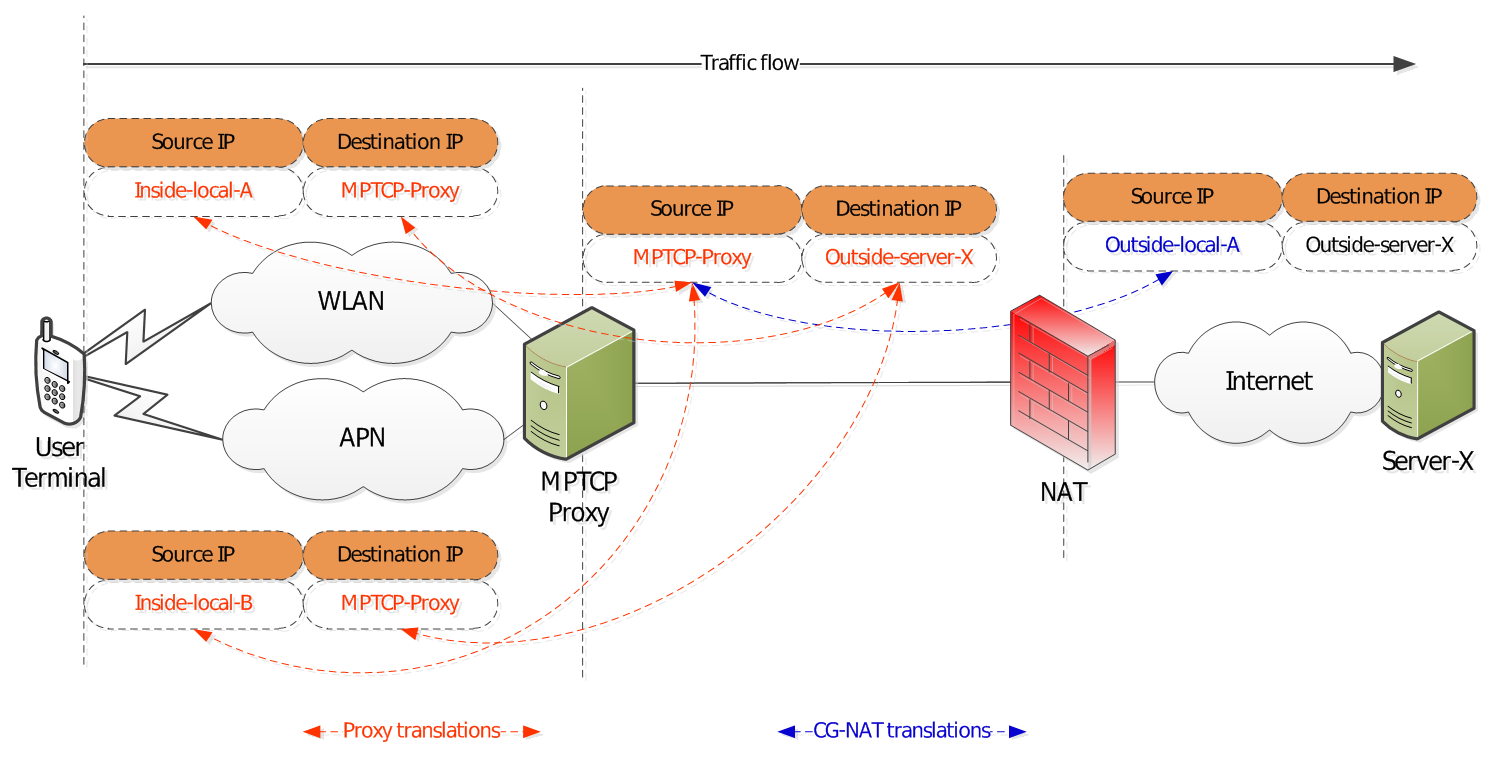
\includegraphics[scale=0.3]{figures/oro/oro_mptcp_nat2.png}
	\caption{Post-proxy NAT}
    	\label{fig:oro_mptcp_nat2}
\end{figure}



\chapter{Arhitectura SOCKS v6}
\label{sec:arch_upb}

% se reia cadrul general cu desenele pentru SOCKSv6

Operatorii de telefonie mobila instaleaza MPTCP \cite{Raiciu_Hard:2012} pe telefoane mobile 
pentru a exploata latimea de banda oferita de LTE si WiFi in acelasi timp. Deoarece foarte putine
servere folosesc MPTCP, este necesar un proxy in incinta operatorului, care sa termine conmexiunea
MPTCP si sa comunice cu serverul folosind TCP normal.

\begin{figure*}[t]
	\centering
	\includegraphics*[angle=0,width=\textwidth]{figures/socks/arch}
	\label{fig:arch}
	\caption{Arhitectura SOCKS v6}
\end{figure*}



\chapter{Caracteristici SOCKS v6}
% spunem despre ce-și doresc mobilele, MPTCP-ul, și securitatea.
% în principiu, ce s-a adăugat în draft-01 șî draft-02
\label{sec:arch_upb}

Versiunile 4 si 5 \cite{rfc1928} ale protocolului SOCKS au fost dezvoltate si standardizate acum
doua decenii si sunt larg folosite in ziua de azi pentru diverse scopuri.
Ele sunt implementate in multe aplicatii, precum browsere web, clienti SSH si proxificatoare.

Este foarte important ca un proxy sa ofere performanta buna si sa profite de cele mai recente
imbunatatiri aduse protocoalelor de retea. Pentru a profita de de TCP Fast Open \cite{rfc7413}
sau pentru oferi securitate mai buna impotriva potentialilor atacatori, Korea Telecom si alti utilizatori
au recurs la proxy-uri precum Shadowsocks \cite{shadowsocks}, care folosesc protocoale nestandardizate
si a caror securitate nu au fost auditata.

Acest capitol descrie versiunea 6 a protocolului SOCKS, care acum este in curs de dezvoltate la IETF \cite{olteanu-intarea-socks-6-02}.
Principala imbunatatire adusa protocolului este eliminarea round-trip-urilor de date dintre client si proxy in cele mai multe cazuri.
SOCKS versiunea 6 rezolva problemele principale ale forlosirii atat TFO, cat si a 0-RTT TLS Session Resumption \cite{tls1.3},
oferind un mecanism care asigura idempotenta cererilor.

SSOCKS v6 este de asemenea extensibil, permitand implementarea unor functionaltiati noi, fara a introduce probleme de compatibilitate.

\section{RTT redus}


\begin{figure*}[t]
	\centering
	\includegraphics*[angle=0,height=.50\textwidth]{figures/socks/a-crop}
	\label{fig:socksv5}
	\caption{SOCKS v5}
\end{figure*}

\begin{figure*}[t]
	\centering
	\includegraphics*[angle=0,height=.50\textwidth]{figures/socks/b-crop}
	\label{fig:socksv6short}
	\caption{SOCKS v6}
\end{figure*}

\begin{figure*}[t]
	\centering
	\includegraphics*[angle=0,height=.50\textwidth]{figures/socks/c-crop}
	\label{fig:yes_yes_no}
	\caption{SOCKS v6 cu TFO disponibil numai intre client si proxy}
\end{figure*}

Atunci cand un client doreste se se conecteze la un server, trebuie sa deschida o conexiune TCP
catre un proxy SOCKS v6. Diferenta principala fata de versiunea 5 este ca se transmit cat mai multe informatii
inca din primul mesaj. Clientul incepe prin a trimite un SOCKS Request, care  contine adresa si
portul serverului, alaturi de o transa initiala de date pentru server (de exemplu, un HTTP GET).
Daca clientul si proxy-ul au comunicat in prealabil, este posibila autentificarea in 0 RTT-uri, caz in care
datele de autentificare sunt si ele incluse in cerere.

Apoi, proxy-ul trimite un Authentication Reply. Daca in Request nu se aflau date de autentificare satisfacatoare,
proxy-ul indica metoda de autentificare ce trebuie sa urmeze. In acest caz, urmeaza o secventa mai lunga de mesaje prin
care clientul se autentifica.

In final, proxy-ul se conecteaza la server si genereaza un Operation Reply, prin indica succesul sau esecul conexiunii.
Datele primite ulterior de proxy sunt trimite verbatim catre capatul celalalt.

In cazul cel mai uzual, in care autentificarea este bine pusa la punct (v. fig. \ref{fig:socksv6short}), proxy-ul
incearca sa se conecteze la server imediat ce promeste Request-ul, neadaugand latenta in plus.

Presupunand ca proxy-ul se afla pe calea dintre client si server, timpul necesar pentru a obtine un raspuns de la server
(de ex. un HTTP OK) prin intermediul SOCKS v6 nu este mai lung decat timpul obtinerii unui raspuns atunci cand serverul
este contactat direct.

\begin{table}
	\centering
	\begin{tabular}{| l | c | c | c | r |} \hline
		& TFO la proxy & TFO la server & RTT total \\ \hline
	% 	SOCKSv5 & \multicolumn{3}{|l|}{~}  & ? 3T + 3t ? \\ \hline
		\multirow{2}{*}{TCP} & - & Nu  & \(2P+2S\) \\ \hhline{~----}
		~ & - & Da  & \(P+S\) \\ \hline
		\multirow{3}{*}{SOCKSv6} & Nu & Nu  & \(2P + 2S\)  \\ \hhline{~----}
		~ & Da & Nu & \(P + 2S\) \\ \hhline{~----}
		~ & Da  & Da & \(P + S\) \\ \hline
	\end{tabular}
  	\caption{Timpul necesar primirii unui raspuns de date. (P = RTT client-proxy, S = RTT proxy-server. P + S = RTT client-server.)}
 \end{table}

SOCKS v6 este \emph{mai rapid} decat TCP atunci cand serverul nu are TFO activat.
Clientii pot folosi TFO pe traseul dintre proxy si server, eliminand un RTT dintre client si proxy.
Acest lucru este foarte avantajos pentru dispozitivele mobile, intrucat latenta dintre dispozitiv si base station
poate fi foarte mare.

In plus, daca rulam SOCKS v6 peste TLS, timpii obtinuti nu se schimba atata timp cat folosim 0-RTT Session Resumption.

Spre diferenta de versiunea 6, in versiunea 5 sunt necesare 2 RTT-uri (sau 3, daca e necesara autentificarea clientilor)
pana cand datele incep sa curga intre client si server.

\section{Operațiuni idempotente cu TLS 1.3}

Atat TCP Fast Open, cat si 0-RTT TLS Session Resumption au probleme bine cunoscute care pot duce la duplicarea unor
cereri din partea clientului.

In cazuri rare, retransmiterea unui SYN cu TFO si date in payload poate duce la creearea unei conexiuni duplicate la server.
Acest lucru poate fi dezastruos daca, de exemplu, serverul se ocupa de tranzactii financiare si proceseaza o tranzactie de doua ori.

In TLS 1.3, un client care deschide o conexiune noua si doreste sa-si continue sesiunea de TLS poate sa includa niste date (de ex. un HTTP GET)
in primul mesaj trimis catre server. Aceste date initiale (numite "Early Data") beneficiaza de securitate mai scazuta.
Daca intre cele doua capete se afla un atacator, acesta poate sa captureze datele initiale (in forma criptata) si sa le foloseasca pentru a creea conexiuni duplicate.

Pentru a folosi in deplina siguranta TFO si 0-RTT Session Resumption intre client si proxy, am implementat un mecanism
prin care se asigura idempotenta cererilor SOCKS. Proxy-ul va onora o cerere individuala cel mult o data, indiferent de cate
ori o primeste.

Pentru a se proteja de cereri duplicate, clientii pot cere, si apoi cheltui, token-uri de idempotenta. Un token poate fi cheltuit pe o singura cerere.

Token-ii sunt intregi fara semn de 4 octeti intr-un spatiu modular de 4 octeti. Astfel, daca \(x\) si \(y\) sunt tokeni, \(x < y\) daca \( 0 < (y - x) < 2^{31} \) (in aritmetica pe 32 de biti).

Proxy-ul acorda intervale contigue de token-uri numite \emph{ferestre}. Aceste ferestre sunt definite de baza (primul token din interval) si de dimensiune.
Ferestrele sunt mutate (adica li se incrementeaza baza, dar isi pastreaza dimensiunea) de catre proxy.

Clientii incearca sa isi cheltuiasca token-urile in ordine. Acest lucru nu garanteaza ca proxy-ul va primi sau va procesa cererile in ordine. De asemenea, unele cereri se pot pierde din cauza retelei.

Proxy-ul urmareste starea tuturor token-ilor din fereastra, mutand fereasta pe masura ce token-urile de la inceputul ferestrei sunt cheltuiti.
Pentru ca un token necheltuit sa nu opreasca avansarea ferestrei, am introdus un parametru numit \emph{high water mark}. Acest parametru
este un numar strict mai mic decat dimensiunea ferestrei. Daca diferenta dintre cel mai mare token cheltuit si cel mai mic token necheltuit este mai
mare decat high water mark, fereastra este mutata si token-ul necheltuit este pierdut. Cresterea acestui parametru face proxy-ul mai tolerant la cereri reordonate.

Mecanismul de idempotenta are urmatoarele proprietati:
\begin{itemize}
    \item \emph{Consum mic de resurse}: Proxy-ul aloca o cantitate fixa de memorie pentru fiecare cliemt. Nu se fac realocari de memorie si toate operatiunile sunt ieftine.
    Mecanismul de idempotenta in sine nu ofera o posibilitate de denial of service.
    \item \emph{Tolerant la crash-uri}: Repornirea proxy-ului va duce la alocarea unei alte ferestre. Din moment ce este foarte improbabil ca
    fereastra noua sa se intersecteze cu chea veche, sansele de a onora o cerere veche sunt foarte mici.
    \item \emph{Sigur}: Pentru a duplica o cerere cu succes, un atacator trebuie sa astepte pana cand fereastra parcurge tot spatiul modular de numere si ajunge inapoi in pozitia initiala
    (adica pana cand clientul face 4 miliarde de cereri).
    \item {Nerestrictiv}: Singura restrictie impusa clientului esre ca poate face un numar limitat de cereri intr-un RTT. Acest lucru nu e o problema daca ferestrele sunt suficient de mari.
\end{itemize}


\section{Opțiuni de configurare a sockeților pe proxy}

Protocolul SOCKS6 dispune de optiuni pentru configurarea socketilor deschisi de proxy.
Pentru o operatiune tipica, un proxy deschide doi socketi: unul pentru a vorbi cu clientul si unul pentru a vorbi cu serverul.

Optiunile de configurare a socketilor au fost modelate pentru a mima semantica functiilor |getsockopt()| si |setsockopt()| si au urmatoarele campuri:

\begin{itemize}
	\item Tronson: client-proxy sau proxy-server.
	\item Nivel: IP generic, IPv4, IPv6, TCP, UDP sau TLS.
	\item Cod: un cod specific operatiunii cerute.
	\item Date: date specifice operatiunii.
\end{itemize}

Clientii pot pune astfel de optiuni intr-un Request pentru a cere un anumit comportament din partea proxy-ului.
De asemenea, proxy-ul poate include astfel de optiuni intr-un Operation Reply pentru a semnaliza comportamentul socketilor sai.

In versiunea curenta a protocolului exista urmatoarele optiuni:
\begin{itemize}
	\item TFO: Clientul poate indica daca doreste ca proxy-ul sa contacteze serverul folosind TFO.
	\item MPTCP: Proxy-ul poate instiinta clientul daca serverul foloseste MPTCP. Astfel, un client mobil poate sa evite folosirea proxy-ului atunci cand contacteaza serverul din nou.
	\item Scheduler MPTCP: Felul in care MPTCP distribuie datele in subflow-uri depinde de un scheduler. In cazul in care un client are o conexiune cu volum mic de date, dar latenta este foarte importanta, poate instrui proxy-ul sa duplice datele pe toate subflow-urile.
\end{itemize}


\chapter{Aplicație de colectare a datelor de la utilizatorii testeri}

\section{Connectivity Manager}
ce face aplicația, o scurtă descriere a feature-lor

link la github 
\section{Structura și utilitatea datelor colectate automat}

datele pe care le colectăm, modul de colectare

utilitarele pe care le folosim, descrise pe scurt (tcp\_ping, etc, doar ce e cazul)

\chapter{Măsurători de handoff folosind terminalul instrumentat}
\section{Arhitectura de test}
cum ai pus mașinile

care e scenariul de intrare, de ieșire

\section{Rezultate măsurători}

grafice comentate


 

%%%%%%%%%%%%%%%%%%%%%%%%%%%%%%%%%%%%%%%%%%%%%%%%%%%%%%%%%%%%%%%%%%%%%-
%% INTRODUCERE - CHAPTER 1
%%%%%%%%%%%%%%%%%%%%%%%%%%%%%%%%%%%%%%%%%%%%%%%%%%%%%%%%%%%%%%%%%%%%%-

% \input{arch-basics}

%\input{faza}
%%%%%%%%%%%%%%%%%%%%%%%%%%%%%%%%%%%%%%%%%%%%%%%%%%%%%%%%%%%%%%%%%%%%%-
%% ARHITECTURA - CHAPTER 2
%%%%%%%%%%%%%%%%%%%%%%%%%%%%%%%%%%%%%%%%%%%%%%%%%%%%%%%%%%%%%%%%%%%%%-
%\input{arhitectura}


%%%%%%%%%%%%%%%%%%%%%%%%%%%%%%%%%%%%%%%%%%%%%%%%%%%%%%%%%%%%%%%%%%%%%-
%% COMPONENTE - CHAPTER 3
%%%%%%%%%%%%%%%%%%%%%%%%%%%%%%%%%%%%%%%%%%%%%%%%%%%%%%%%%%%%%%%%%%%%%-

% \chapter*{SECTIUNEA I: Stabilirea Cerintelor si Modelului Arhitectural}
% 
% \addcontentsline{toc}{chapter}{SECTIUNEA I: Stabilirea Cerintelor si Modelului Arhitectural}
% 
% \input{middlebox_study}
% 
% \input{componente}
% 
% 
% \chapter*{SECTIUNEA II: Proiectarea Platformei si Protocoalelor}
% \addcontentsline{toc}{chapter}{SECTIUNEA II: Proiectarea Platformei si Protocoalelor}
% \input{platforma}


%%%%%%%%%%%%%%%%%%%%%%%%%%%%%%%%%%%%%%%%%%%%%%%%%%%%%%%%%%%%%%%%%%%%%-
%% Aplicatii - CHAPTER 5
%%%%%%%%%%%%%%%%%%%%%%%%%%%%%%%%%%%%%%%%%%%%%%%%%%%%%%%%%%%%%%%%%%%%%-
% \input{aplicatii}

%%%%%%%%%%%%%%%%%%%%%%%%%%%%%%%%%%%%%%%%%%%%%%%%%%%%%%%%%%%%%%%%%%%%%-
%% Concluzii - CHAPTER 6
%%%%%%%%%%%%%%%%%%%%%%%%%%%%%%%%%%%%%%%%%%%%%%%%%%%%%%%%%%%%%%%%%%%%%-
% \chapter{Concluzii}
% \input{concluzii}
% 
% \chapter*{SECTIUNEA III: Stabilirea Planului de Diseminare}
% \input{dissemination}
% 
% \addcontentsline{toc}{chapter}{SECTIUNEA III: Stabilirea Planului de Diseminare}


%%%%%%%%%%%%%%%%%%%%%%%%%%%%%%%%%%%%%%%%%%%%%%%%%%%%%%%%%%%%%%%%%%%%%-
%% BIBLIOGRAPHY
%%%%%%%%%%%%%%%%%%%%%%%%%%%%%%%%%%%%%%%%%%%%%%%%%%%%%%%%%%%%%%%%%%%%%-
\addcontentsline{toc}{chapter}{Bibliografie}
\renewcommand{\bibname}{Bibliografie}

\addcontentsline{toc}{chapter}{References}
%\bibliographystyle{ieeetr}
\bibliographystyle{plain}
%\bibliographystyle{abbrv}
%\bibliographystyle{phjcp}
%%\bibliographystyle{apalike}
\bibliography{references}
% \bibliography{chapters/symnet/biblio}
%%%%%%%%%%%%%%%%%%%%%%%%%%%%%%%%%%%%%%%%%%%%%%%%%%%%%%%%%%%%%%%%%%%%%%
%%% content.tex ends here


%%%%%%%%%%%%%%%%%%%%%%%%%%%%%%%%%%%%%%%%%%%%%%%%%%%%%%%%%%%%%%%%%%%%%%%%
%                   End the document
%%%%%%%%%%%%%%%%%%%%%%%%%%%%%%%%%%%%%%%%%%%%%%%%%%%%%%%%%%%%%%%%%%%%%%%%
\end{document}

%%%%%%%%%%%%%%%%%%%%%%%%%%%%%%%%%%%%%%%%%%%%%%%%%%%%%%%%%%%%%%%%%%%%%%
%%% main.tex ends here

